
\begin{comment}
\documentclass{article}
\usepackage[utf8]{inputenc}
\usepackage{graphicx}
\usepackage{hyperref}
\usepackage{float}


\DeclareGraphicsExtensions{.jpg}
\graphicspath{{./Images/}}

\end{comment}
	
\begin{titlepage}
\begin{center}

\includegraphics[width = 0.3\textwidth]{US_logo.png}~\\[1cm]
\textsc{\LARGE Unsolvable Solutions}\\
Client: Francois Mouton at the CSIR DSSR\\[1.5cm]
\textsc{\Large  User Manual}\\[0.5cm]

 \HRule\\[0.4cm]
{ \huge \bfseries  Eavesdropping Protection in Conclave \\[0.4cm] }

 \HRule\\ 



Github link:  \url{https://github.com/Unsolvable-Solutions/Project-EPIC} \\[1.2cm]

\noindent
\begin{minipage}[t]{0.4\textwidth}

	\begin{flushleft} \large
	\emph{Members:}\\
		Edwin Fullard  \\
		Jaco Bezuidenhoudt \\
		Jandre Coetzee\\
		Maret Stoffberg\\
		Ryno Pierce\\
	\end{flushleft}
\end{minipage}%
\begin{minipage}[t]{0.4\textwidth}
\begin{flushright} \large
	\emph{Student Number:} \\
		12048675 \\
		11013878 \\
		 10693077 \\
		 11071762 \\
		 12003922\\
	\end{flushright}
\end{minipage}

\vfill


% Bottom of the page




\end{center}
\end{titlepage}

	
	% Table of content
	\newpage
	\tableofcontents
	\newpage
	\section{Introduction}
	\subsection{Project Background}

The Android Operating System officially took over the smart phone market in 2010 and it is suspected that about 700 000 Android devices are used in South Africa. It is mostly the corporate or more upper class communities that use these smart phone devices. It is also these individuals who sit in the big corporate meetings where extremely sensitive data can be discussed. For this reason, if these individuals could have eavesdropping malware on their smart phone, it could cause sensitive data to be easily leaked out.


	\subsection{Project Vision} 
	The Eavesdropping Protection in Conclave (EPIC) aims to protect the integrity of the information discussed during a meeting by eliminating access to the mobile device during a meeting.

	\subsection{Project Scope}
		The Eavesdropping Protection in Conclave(EPIC) product consist of a mobile application, a web page, a server, a gateway and a node. 
		\begin{itemize}
		\item A meeting is scheduled via the web page. On the creation of the meeting people are invited via email.
		\item Before the meeting is held, the gateway and node is set up with the list of invited people that may access the meeting room.
		\item At the meeting, the person opens the application on his phone. He then holds the phone over the node. The node then replies if the person has permission to access the room or not. If the person has permission the meeting room is unlocked.
		\item If access is denied, the gateway sends a refresh request to the server, and the person can try again to gain access.
		\item When permission is granted, the application will start the protecting mode on the phone.
		\item The server keeps a log of all the activities. This log can be queried afterwards by the creator of the meeting.
        \end{itemize}



	%  The functional requirements
\newpage
\section{Functional Requirements}

	\begin{comment}
Template vir elke funksie
    \paragraph{Funksie naam}
			\begin{description}
			    \item{\textbf{Priority}:} %watter prioriteit dit het: Critical, Important of Nic-to-have
			    \item{\textbf{Service Contract}:}% Wat dit doen
			    \item{\textbf{Pre-conditions}:}%wat moet waar wees voor die funksie sy ding kan doen
    			    \begin{itemize}
    			        \item %precondition 1
    			        \item %precondition 2
    			    \end{itemize}
			    \item{\textbf{Post-conditions}:} % wat moet waar wees na die funksie sy ding gedoen het
    			    \begin{itemize}
    			    \item %post condition 1
    			    \item %post condition2
    			    \end{itemize}
			\end{description}
\end{comment}








	\subsection{Server}
	    \subsubsection{Scope: }
	    \begin{itemize}
	    \item The server is used with the gateway: it sends and receives data to and from the server. 
	    \item A user can add, remove and edit meetings on the server via the website.
	    \item A user can add people to a meeting and remove people from a meeting on the server via the website.
	    \item The server stores a database with all the data.
	    \end{itemize}

%		\begin{figure}[H]
 %			 \centering
%			  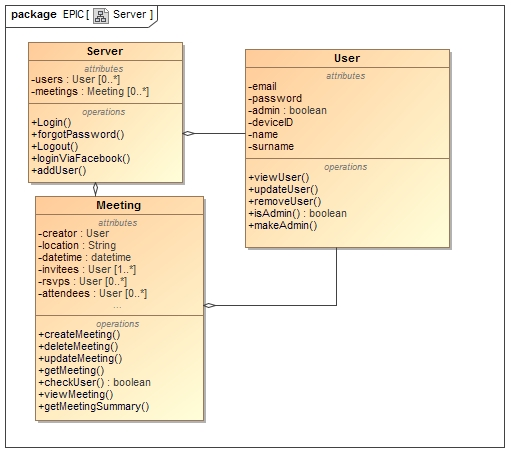
\includegraphics[width=12cm]{ServerClass}
%		 	 \caption{A Class Diagram of the Server}
%		\end{figure}
		
		
		
		\subsubsection{Functionality}
		
		    \paragraph{getMeeting}
			\begin{description}
			    \item{\textbf{Priority}:} Critical%watter prioriteit dit het: Critical, Important of Nic-to-have
			    \item{\textbf{Service Contract}:} A query is made for a specific meeting and the function returns a JSON object with the meeting that meet the query. 
			    \item{\textbf{Pre-conditions}:}%wat moet waar wees voor die funksie sy ding kan doen
    			    \begin{itemize}
    			        \item The query must be valid.
    			        \item The meeting must exist.
    			    \end{itemize}
			    \item{\textbf{Post-conditions}:} % wat moet waar wees na die funksie sy ding gedoen het
    			    \begin{itemize}
    			    \item A meeting object that meet the query is returned. 
    			    \item The action is logged on the server.
    			    \end{itemize}
			\end{description}
	

		    \paragraph{getPeopleList}
			\begin{description}
			    \item{\textbf{Priority}:} Critical%watter prioriteit dit het: Critical, Important of Nic-to-have
			    \item{\textbf{Service Contract}:} This function returns a list of Person object that may attend a specified meeting.
			    \item{\textbf{Pre-conditions}:}%wat moet waar wees voor die funksie sy ding kan doen
    			    \begin{itemize}
    			        \item The meeting must be specified.
    			        \item The meeting must exist.%precondition 1
    			        \item Only the owner of the meeting or the gateway may call this function. \item The server must be running.%precondition 2
    			    \end{itemize}
			    \item{\textbf{Post-conditions}:} % wat moet waar wees na die funksie sy ding gedoen het
    			    \begin{itemize}
    			    \item A list of Person objects is returned.%post condition 1
    			    \item The action is logged.%post condition2
    			    \end{itemize}
			\end{description}
			

    \paragraph{Create Person}
			\begin{description}
			    \item{\textbf{Priority}:} Critical %watter prioriteit dit het: Critical, Important of Nice-to-have
			    \item{\textbf{Service Contract}:} This function is called when a person is added to a meetings people list and the person is not yet in the database. The function creates a Person object and stores it in the database.
			    \item{\textbf{Pre-conditions}:}%wat moet waar wees voor die funksie sy ding kan doen
    			    \begin{itemize}
    			        \item The user must have permission to add the person.
    			        \item The required fields are email address, name and surname.
    			    \end{itemize}
			    \item{\textbf{Post-conditions}:} % wat moet waar wees na die funksie sy ding gedoen het
    			    \begin{itemize}
    			    \item The person object is created and it is added to the database.
    			    \item The action is logged in the database.
    			    \end{itemize}
			\end{description}
    

    \paragraph{Create meeting}
			\begin{description}
			    \item{\textbf{Priority}:} Critical%watter prioriteit dit het: Critical, Important of Nic-to-have
			    \item{\textbf{Service Contract}:} The function is called by the website when the user creates a meeting. The meeting object is then created and stored in the database.% Wat dit doen
			    \item{\textbf{Pre-conditions}:}%wat moet waar wees voor die funksie sy ding kan doen
    			    \begin{itemize}
    			        \item The meeting title, meeting room, date and time are required fields.
    			    \end{itemize}
			    \item{\textbf{Post-conditions}:} % wat moet waar wees na die funksie sy ding gedoen het
    			    \begin{itemize}
    			    \item The meeting object is created and it is added to the database.
    			    \item The action is logged in the database.
    			    \end{itemize}
			\end{description}

    \begin{comment}
Template vir elke funksie
    \paragraph{Funksie naam}
			\begin{description}
			    \item{\textbf{Priority}:} %watter prioriteit dit het: Critical, Important of Nic-to-have
			    \item{\textbf{Service Contract}:}% Wat dit doen
			    \item{\textbf{Pre-conditions}:}%wat moet waar wees voor die funksie sy ding kan doen
    			    \begin{itemize}
    			        \item %precondition 1
    			        \item %precondition 2
    			    \end{itemize}
			    \item{\textbf{Post-conditions}:} % wat moet waar wees na die funksie sy ding gedoen het
    			    \begin{itemize}
    			    \item %post condition 1
    			    \item %post condition2
    			    \end{itemize}
			\end{description}
\end{comment}






\subsection{Website}


	\subsubsection{Scope}
	The website is used by a user to manage his meetings. 
	
	\subsubsection{Functionality}
	
    	\paragraph{Register}
			\begin{description}
			    \item{\textbf{Priority}:} Important
			    \item{\textbf{Service Contract}:} The user enters his name, surname, email address and password. These details are stored in the database on the server and the user is automatically logged in.
			    \item{\textbf{Pre-conditions}:}%wat moet waar wees voor die funksie sy ding kan doen
    			    \begin{itemize}
    			        \item The user must be connected to the Internet.
    			        \item The server must running.
    			    \end{itemize}
			    \item{\textbf{Post-conditions}:} % wat moet waar wees na die funksie sy ding gedoen het
    			    \begin{itemize}
    			    \item The users name, surname, email address and password are stored in the database. 
    			    \item login function is called with the users details.
    			    \item  The action is logged in the database.
    			    \end{itemize}
			\end{description}
	
	\begin{figure}[H]	
 			 \centering
			  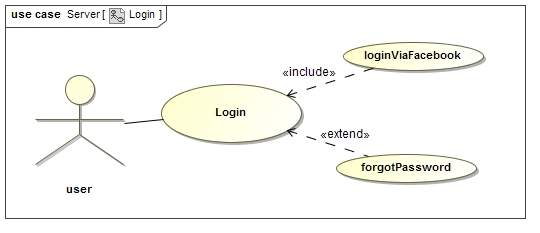
\includegraphics[width=12cm]{LoginUseCase}
		 	 \caption{A Use Case Diagram of the Login services}
		\end{figure}
    	\paragraph{Log in}
			\begin{description}
			    \item{\textbf{Priority}:} Important
			    \item{\textbf{Service Contract}:}The user types his email address and password to enter the website
			    \item{\textbf{Pre-conditions}:}%wat moet waar wees voor die funksie sy ding kan doen
    			    \begin{itemize}
    			        \item The browser must be connected to the Internet.
    			        \item The server must running.
    			        \item The user must be registered.
    			        \item The password must be correct.
    			    \end{itemize}
			    \item{\textbf{Post-conditions}:}
    			    \begin{itemize}
    			    \item The user becomes the current user on the website session.%sê beter
    			    \item The user is on his home page.
    			    \item  The action is logged in the database.
    			    
    			    \end{itemize}
			\end{description}
			
    	\paragraph{Log out}
			\begin{description}
			    \item{\textbf{Priority}:} Important
			    \item{\textbf{Service Contract}:} The user clicks on a button and the user is logged out of his account. 
			    \item{\textbf{Pre-conditions}:}
    			    \begin{itemize}
    			        \item The browser must be connected to the Internet.
    			        \item The server must running. 	
    			        \item The user has to be logged in. 
    			    \end{itemize}
			    \item{\textbf{Post-conditions}:} 
    			    \begin{itemize}
    			      \item The user is logged out.
    			      \item The current user on the session becomes null.
    			      \item The browser is redirected to the log in page 
    			      \item  The action is logged in the database.
    			    \end{itemize}
			\end{description}
			
    	\paragraph{Reset password}
			\begin{description}
			    \item{\textbf{Priority}:} Nice to Have
			    \item{\textbf{Service Contract}:} The user can reset a forgotten password. The function is available on the log in page. 
			    \item{\textbf{Pre-conditions}:}
    			    \begin{itemize}
    			        \item The browser must be connected to the Internet.
    			        \item The server must running. 	
    			        \item The user should not be logged in. 
    			        \item The user has to provide an email address.
    			    \end{itemize}
			    \item{\textbf{Post-conditions}:} 
    			    \begin{itemize}
    			      \item An email is send to the users email address with a link to the reset password web page. The user has to open it.
    			      \item On the reset password page, the user enters the password twice.
    			      \item The users password is changed in the database.
    			      \item The user is redirected to the log in page.
    			      \item  The action is logged in the database.
    			    \end{itemize}
			\end{description}
							
			
    	\paragraph{Create Meeting}
			\begin{description}
			    \item{\textbf{Priority}:} Critical
			    \item{\textbf{Service Contract}:} The user schedules a meeting by entering the title, description, meeting room, time and date.
			    \item{\textbf{Pre-conditions}:}
    			    \begin{itemize}
    			        \item The browser must be connected to the Internet.
    			        \item The server must running.    		  
    			        \item The user has to be logged in. 
    			        \item The meeting title, meeting room, date and time are required fields.
    			    \end{itemize}
			    \item{\textbf{Post-conditions}:} 
    			    \begin{itemize}
    			      \item The meeting and its details are stored in the database.
    			      \item The meeting is  added to the users list of meetings on the database. 
    			      \item The update meeting, invite person and remove meeting functions are available. 
    			      \item  The action is logged in the database. 
    			    \end{itemize}
			\end{description}
			
    	\paragraph{Invite Person}
			\begin{description}
			    \item{\textbf{Priority}:} Critical
			    \item{\textbf{Service Contract}:} The user invites a person to a specific meeting. This function is called for every person being invited.
			    \item{\textbf{Pre-conditions}:}
    			    \begin{itemize}
    			        \item The browser must be connected to the Internet.
    			        \item The server must running.	        
    			        \item The user has to be logged in. 
    			        \item The meeting has to be specified.
    			        \item The required fields for the person being invited are: the name, surname and email address.
    			    \end{itemize}
			    \item{\textbf{Post-conditions}:} 
    			    \begin{itemize}
    			      \item If the person does not yet exist in the database he is added to the database.
    			      \item The person is added to the meetings list of invited people. 
    			      \item An email is send to the person to notify him of the meeting.
    			      \item The action is logged in the database.
    			    \end{itemize}
			\end{description}	
			
    	\paragraph{Remove Person}
			\begin{description}
			    \item{\textbf{Priority}:} Important
			    \item{\textbf{Service Contract}:} The user removes a person from the list of invited people of a specified meeting.
			    \item{\textbf{Pre-conditions}:}
    			    \begin{itemize}
    			        \item The browser must be connected to the Internet.
    			        \item The server must running.    	       
    			        \item The user has to be logged in. 
    			        \item The meeting has to be specified.
    			        \item The person has to be specified.
    			        \item The person has to exist in the meetings list of invited people.
    			        \item The user has to confirm the action.
    			    \end{itemize}
			    \item{\textbf{Post-conditions}:} 
    			    \begin{itemize}
    			      \item The person is removed from the list of invited people of the meeting.
    			      \item The person is not removed from the database. 
    			      \item An email is send to the person to notify him that he has been removed from the list.
    			      \item The action is logged in the database.
    			    \end{itemize}
			\end{description}	
			
    	\paragraph{Update Meeting}
			\begin{description}
			    \item{\textbf{Priority}:} Important
			    \item{\textbf{Service Contract}:} The user can update any of the specified meetings fields.
			    \item{\textbf{Pre-conditions}:}
    			    \begin{itemize}
    			        \item The browser must be connected to the Internet.
    			        \item The server must running.
    			        \item The user has to be logged in. 
    			        \item The meeting has to be specified.
    			    \end{itemize}
			    \item{\textbf{Post-conditions}:} 
    			    \begin{itemize}
    			      \item The change is made to the meeting in the database.
    			      \item The action is logged in the database.
    			    \end{itemize}
			\end{description}	
	    
	    \paragraph{Remove Meeting}
			\begin{description}
			    \item{\textbf{Priority}:} Important %watter prioriteit dit het: Critical, Important of Nic-to-have
			    \item{\textbf{Service Contract}:} The specified meeting is logically removed from the database.% Wat dit doen
			    \item{\textbf{Pre-conditions}:}%wat moet waar wees voor die funksie sy ding kan doen
    			    \begin{itemize}
    			        \item The browser must be connected to the Internet.
    			        \item The server must running.
    			        \item The user has to be logged in. 
    			        \item The meeting has to be specified.
    			    \end{itemize}
			    \item{\textbf{Post-conditions}:} % wat moet waar wees na die funksie sy ding gedoen het
    			    \begin{itemize}
    			    \item All the invited people are notified via email.
    			    \item The meeting is no on the owners list of meetings.
    			    \item The meeting is no longer on the invited peoples list of meetings.
    			    \item The action is logged in the databases.
    			    \end{itemize}
			\end{description}
			
					
							
			

    \begin{comment}
Template vir elke funksie
    \paragraph{Funksie naam}
			\begin{description}
			    \item{\textbf{Priority}:} %watter prioriteit dit het: Critical, Important of Nic-to-have
			    \item{\textbf{Service Contract}:}% Wat dit doen
			    \item{\textbf{Pre-conditions}:}%wat moet waar wees voor die funksie sy ding kan doen
    			    \begin{itemize}
    			        \item precondition 1
    			        \item precondition 2
    			    \end{itemize}
			    \item{\textbf{Post-conditions}:} % wat moet waar wees na die funksie sy ding gedoen het
    			    \begin{itemize}
    	    	    \item %post condition 1
    			    \item %post condition2
    			    \end{itemize}
			\end{description}
\end{comment}









\subsection{Application}
		\subsubsection{Scope}
		    The Application is used when entering a meeting. 
		    \begin{itemize}
		    \item The user will hold the mobile device over a node.
		    \item The application will send the device identification and the persons email address to the gateway via the node. 
    		    \begin{description}
    		        \item{\textbf{If permission is granted}:} The background of the application will turn green and the application will take a snapshot of the mobile device's current state and enable the protection. The snapshot is taken so that the mobile Device and application can be restored to its previous state after the meeting.
    		        \item{\textbf{If permission is denied}:} The background of the application will  turn red and the application will do nothing.
    		        
    		    \end{description}
		    \item During the meeting the application check constantly if the protection mode is violated. If so, the protection mode is restored and the mobile device vibrates to alert the user of a possible attack.
		    \item When exiting the meeting the user holds the mobile device over the node again and the mobile device is restored to its previous state.
		    \item{ Overall system layout: 
		    
		    

		
		\begin{figure}[H]
 			 \centering
			  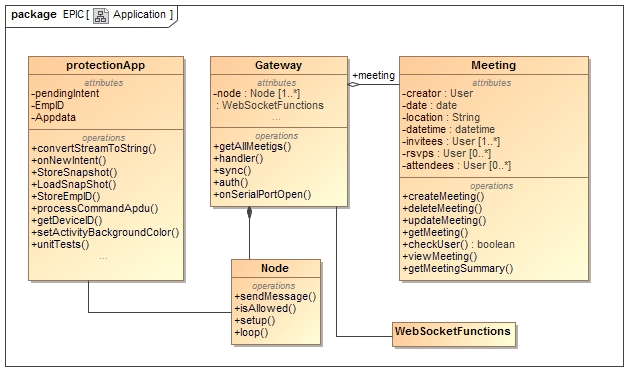
\includegraphics[width=12cm]{ApplicationClass}
		 	 \caption{A Class Diagram of the protection Application, Meeting, Node and Gateway}
		\end{figure}}
		\end{itemize}
       
       
        \subsubsection{Functionality}

		\begin{figure}[H]
 			 \centering
			  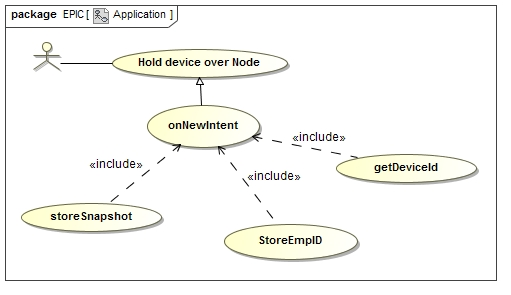
\includegraphics[width=12cm]{ApplicationUseCase}
		 	 \caption{A Use Case Diagram protection Application}
		\end{figure}


    \paragraph{onNewIntent}
			\begin{description}
			    \item{\textbf{Priority}:} Critical%watter prioriteit dit het: Critical, Important of Nic-to-have
			    \item{\textbf{Service Contract}:}This function is called when an Android system intent is triggered. It checks whether the intent was caused by NFC and then parses the NFC message that will check whether the user is allowed to enter the room. If the user is allowed, the store- and loadSnapshot functions are called respectively on whether the user is entering or leaving.% Wat dit doen
			    \item{\textbf{Pre-conditions}:}%wat moet waar wees voor die funksie sy ding kan doen
    			    \begin{itemize}
    			        \item An NFC intent must be triggered by holding the mobile device against a node.
    			        \item Application either in safe or unsafe mode.
      			    \end{itemize}
			    \item{\textbf{Post-conditions}:} % wat moet waar wees na die funksie sy ding gedoen het
    			    \begin{itemize}
    		        \item According to the state of the application, either the LoadSnapshot or StoreSnapshot function should be called.
    			    
    			    \end{itemize}
			\end{description}
	

	    \paragraph{StoreSnapshot}
			\begin{description}
			    \item{\textbf{Priority}:} Critical
			    \item{\textbf{Service Contract}:} This function stores the state of all communication mechanisms and then turns them off to enter \textit{protection mode}.
			    \item{\textbf{Pre-conditions}:}
    			    \begin{itemize}
    			        \item The mobile device must have enough space to store the file with all the states. 
    			        \item The mobile application must be in the unsafe state.
    			    \end{itemize}
			    \item{\textbf{Post-conditions}:} 
    			    \begin{itemize}
    			    \item A file is stored containing the current states of the mobile device's communication mechanisms.
    			    \item All communication mechanisms are turned off.
    			    \item The mobile application's state is switched to safe mode. 
    			    \end{itemize}
			\end{description}
			
	    \paragraph{LoadSnapShot}
			\begin{description}
			    \item{\textbf{Priority}:} Critical%watter prioriteit dit het: Critical, Important of Nic-to-have
			    \item{\textbf{Service Contract}:} This function is an overwritten function. It is used to create the user authentication data and return it when the mobile device is being read from via NFC.% Wat dit doen
			    \item{\textbf{Pre-conditions}:}%wat moet waar wees voor die funksie sy ding kan doen
    			    \begin{itemize}
    			        \item The mobile application should be in the safe state.
    			        \item The connections should not have been toggled on while in safe state.
  
    			    \end{itemize}
			    \item{\textbf{Post-conditions}:} % wat moet waar wees na die funksie sy ding gedoen het
    			    \begin{itemize}
    			    \item The mobile application is switched to unsafe state.
    			    \item The connections of the mobile device are restored based on previous unsafe state.

    			    \end{itemize}
			\end{description}	
			
				
		\paragraph{StoreEmpID}
			\begin{description}
			    \item{\textbf{Priority}:} Critical %watter prioriteit dit het: Critical, Important of Nic-to-have
			    \item{\textbf{Service Contract}:}This function stores a combination of fields entered by the user into a file that is used to with other functions to either retrieve the data if the application is closed and reopen, or send it via NFC to get use as authentication.% Wat dit doen
			    \item{\textbf{Pre-conditions}:}%wat moet waar wees voor die funksie sy ding kan doen
    			    \begin{itemize}
    			        \item The Employee ID text field should not be empty.
    			        \item The ID needs to be valid.
    			        \item The mobile device needs to have enough space to store a file.

    			    \end{itemize}
			    \item{\textbf{Post-conditions}:} % wat moet waar wees na die funksie sy ding gedoen het
    			    \begin{itemize}
    			    \item A file containing the Employee ID is stored to the local mobile device.
    			    \end{itemize}
			\end{description}	
				
		\paragraph{getDeviceId}
			\begin{description}
			    \item{\textbf{Priority}:} Important%watter prioriteit dit het: Critical, Important of Nic-to-have
			    \item{\textbf{Service Contract}:} Used to added an extra security layer to authentication by getting the unique device id.% Wat dit doen
			    \item{\textbf{Pre-conditions}:}%wat moet waar wees voor die funksie sy ding kan doen
    			    \begin{itemize}
    			        \item The mobile device must be a valid device and have a unique id.
    			    \end{itemize}
			    \item{\textbf{Post-conditions}:} % wat moet waar wees na die funksie sy ding gedoen het
    			    \begin{itemize}
    			    \item The state of the mobile application should be unchanged.
    			    \end{itemize}
			\end{description}	
			
		\paragraph{unitTests}
			\begin{description}
			    \item{\textbf{Priority}:} Critical %watter prioriteit dit het: Critical, Important of Nic-to-have
			    \item{\textbf{Service Contract}:}This function uses dummy scenario's to test whether all of the functions work as they should.% Wat dit doen
			    \item{\textbf{Pre-conditions}:}%wat moet waar wees voor die funksie sy ding kan doen
    			    \begin{itemize}
    			        \item The mobile application must be in debugging mode.
    			        \item The mobile application must be in the unsafe state.
    			        \item The mobile application must have enough space to store the results.
    			    \end{itemize}
			    \item{\textbf{Post-conditions}:} % wat moet waar wees na die funksie sy ding gedoen het
    			    \begin{itemize}
    			    \item The mobile application should be in the unsafe state.
    			    \item A file with the unit test results is stored to the mobile device.
    			    \end{itemize}
			\end{description}

				
		\paragraph{setActivityBackgroundColor}
			\begin{description}
			    \item{\textbf{Priority}:} Nice to have%watter prioriteit dit het: Critical, Important of Nic-to-have
			    \item{\textbf{Service Contract}:} This function changes the background colour of the application to visually notify the user if he has been granted access to the meeting room.% Wat dit doen
			    \item{\textbf{Pre-conditions}:}%wat moet waar wees voor die funksie sy ding kan doen
    			    \begin{itemize}
    			        \item The state of the application needs to be changed.
    			    \end{itemize}
			    \item{\textbf{Post-conditions}:} % wat moet waar wees na die funksie sy ding gedoen het
    			    \begin{itemize}
    			    \item The mobile application's background colour should be the new colour.
    			    \end{itemize}
			\end{description}
			
		\paragraph{convertStreamToString}
			\begin{description}
			    \item{\textbf{Priority}:} Nice to have%watter prioriteit dit het: Critical, Important of Nic-to-have
			    \item{\textbf{Service Contract}:} This function helps to convert an input stream of bytes into a \textit{String type} that is used for file reading.% Wat dit doen
			    \item{\textbf{Pre-conditions}:}%wat moet waar wees voor die funksie sy ding kan doen
    			    \begin{itemize}
    			        \item The input stream must be given
    		%	        \item %precondition 2
    			    \end{itemize}
			    \item{\textbf{Post-conditions}:} % wat moet waar wees na die funksie sy ding gedoen het
    			    \begin{itemize}
    			    \item The function returns a String object containing the value of the stream converted to a String data type. 
    		%	    \item %post condition2
    			    \end{itemize}
			\end{description}




	\begin{comment}
Template vir elke funksie
    \paragraph{Funksie naam}
			\begin{description}
			    \item{\textbf{Priority}:} %watter prioriteit dit het: Critical, Important of Nic-to-have
			    \item{\textbf{Service Contract}:}% Wat dit doen
			    \item{\textbf{Pre-conditions}:}%wat moet waar wees voor die funksie sy ding kan doen
    			    \begin{itemize}
    			        \item %precondition 1
    			        \item %precondition 2
    			    \end{itemize}
			    \item{\textbf{Post-conditions}:} % wat moet waar wees na die funksie sy ding gedoen het
    			    \begin{itemize}
    			    \item %post condition 1
    			    \item %post condition2
    			    \end{itemize}
			\end{description}
\end{comment}






\subsection{Node}
    \subsubsection{Scope:} 
    \begin{itemize}
    \item The node is connected to the gateway with a serial connection.
    \item The node uses NFC to communicate with the Protection App on the phone.
    \item When the phone is scanned, it sends the device id of the phone to the node. The node then sends it to the gateway to verify if the user has access to the meeting. When the gateway replies with the results of the verification, the node turns the lights the appropriate colour, decides if the door must be unlocked and sends feedback to the phone.
    
    \end{itemize} 
    
    \begin{figure}[H]
 			 \centering
			  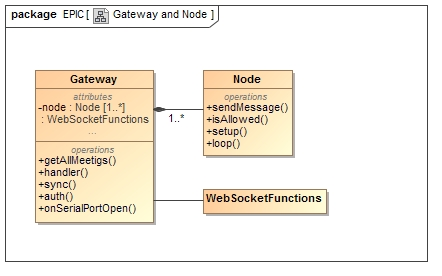
\includegraphics[width=12cm]{GatewayAndNodeClass}
		 	 \caption{A Class Diagram of the Gateway and Node}
		\end{figure}
		
    \subsubsection{Functionality}
        \paragraph{isAllowed}
			\begin{description}
			    \item{\textbf{Priority}:} Critical%watter prioriteit dit het: Critical, Important of Nic-to-have
			    \item{\textbf{Service Contract}:} Sends the device ID to the Gateway and waits until it receives the results on whether or not to allow the user in.% Wat dit doen
			    \item{\textbf{Pre-conditions}:}%wat moet waar wees voor die funksie sy ding kan doen
    			    \begin{itemize}
    			        \item The users' phone should be on the Node.
    			        \item The Protection App should have sent the device ID.
    			    \end{itemize}
			    \item{\textbf{Post-conditions}:} % wat moet waar wees na die funksie sy ding gedoen het
    			    \begin{itemize}
    			        \item The Gateway should have sent a reply.
    			        \item The sendMessage function should be called.
    			    \end{itemize}
			\end{description}

        \paragraph{sendMessage}
			\begin{description}
			    \item{\textbf{Priority}:} Critical%watter prioriteit dit het: Critical, Important of Nic-to-have
			    \item{\textbf{Service Contract}:} This function adapts the results to the correct format that the Protection App is expecting, and then broadcasts it via NFC to the phone. It also calls the setColor function with the appropriate values and calls the openDoor function if the user is allowed in the meeting.
			    \item{\textbf{Pre-conditions}:}%wat moet waar wees voor die funksie sy ding kan doen
    			    \begin{itemize}
    			        \item The results from the Gateway should be received.
    			        \item The users' phone should still be on the Node.
    			    \end{itemize}
			    \item{\textbf{Post-conditions}:} % wat moet waar wees na die funksie sy ding gedoen het
    			    \begin{itemize}
    			        \item The Protection App should have received the results.
    			        \item The lights should reflect the colour of the results.
    			        \item The door should be unlocked if the lights turned green.
    			    \end{itemize}
			\end{description}
		
        \paragraph{setColor}
			\begin{description}
			    \item{\textbf{Priority}:} Important%watter prioriteit dit het: Critical, Important of Nic-to-have
			    \item{\textbf{Service Contract}:} This function receives an RGB colour value and sets the lights to turn that colour. 
			    \item{\textbf{Pre-conditions}:}%wat moet waar wees voor die funksie sy ding kan doen
    			    \begin{itemize}
    			        \item The lights should have power.
    			    \end{itemize}
			    \item{\textbf{Post-conditions}:} % wat moet waar wees na die funksie sy ding gedoen het
    			    \begin{itemize}
    			        \item The lights should be the desired colour.
    			    \end{itemize}
			\end{description}
			
		\paragraph{openDoor}
			\begin{description}
			    \item{\textbf{Priority}:} Nice-to-have%watter prioriteit dit het: Critical, Important of Nic-to-have
			    \item{\textbf{Service Contract}:} This function unlocks the door temporarily so that the user can enter the meeting room.
			    \item{\textbf{Pre-conditions}:}%wat moet waar wees voor die funksie sy ding kan doen
    			    \begin{itemize}
    			        \item The door should be locked.
    			        \item The user must be in front of the door.
    			    \end{itemize}
			    \item{\textbf{Post-conditions}:} % wat moet waar wees na die funksie sy ding gedoen het
    			    \begin{itemize}
    			        \item The door should be locked again.
    			        \item The user must be on the other side of the door.
    			    \end{itemize}
			\end{description}
			
		\paragraph{waiting}
			\begin{description}
			    \item{\textbf{Priority}:} Important%watter prioriteit dit het: Critical, Important of Nic-to-have
			    \item{\textbf{Service Contract}:} Runs the lights through a sequence and delays the loop function a bit. 
			    \item{\textbf{Pre-conditions}:}%wat moet waar wees voor die funksie sy ding kan doen
    			    \begin{itemize}
    			        \item None
    			    \end{itemize}
			    \item{\textbf{Post-conditions}:} % wat moet waar wees na die funksie sy ding gedoen het
    			    \begin{itemize}
    			        \item None
    			    \end{itemize}
			\end{description}
			
		\paragraph{setup}
			\begin{description}
			    \item{\textbf{Priority}:} Critical%watter prioriteit dit het: Critical, Important of Nic-to-have
			    \item{\textbf{Service Contract}:} Initialises the necessary variables and objects and starts the loop function. 
			    \item{\textbf{Pre-conditions}:}%wat moet waar wees voor die funksie sy ding kan doen
    			    \begin{itemize}
    			        \item The Node should be plugged in.
    			    \end{itemize}
			    \item{\textbf{Post-conditions}:} % wat moet waar wees na die funksie sy ding gedoen het
    			    \begin{itemize}
    			        \item The necessary variables and objects should be created in memory.
    			        \item The loop function should have been called.
    			    \end{itemize}
			\end{description}


		 \paragraph{loop}
			\begin{description}
			    \item{\textbf{Priority}:} Critical%watter prioriteit dit het: Critical, Important of Nic-to-have
			    \item{\textbf{Service Contract}:} Gets automatically called over and over like an infinite loop. Each time this function executes it calls the waiting function and then checks for input from the NFC board. When a valid identifier is received, it calls the sendMessage function with the results from the isAllowed function.
			    \item{\textbf{Pre-conditions}:}%wat moet waar wees voor die funksie sy ding kan doen
    			    \begin{itemize}
    			        \item The setup function should have succesfuly completed.
    			    \end{itemize}
			    \item{\textbf{Post-conditions}:} % wat moet waar wees na die funksie sy ding gedoen het
    			    \begin{itemize}
    			        \item Either Nothing should have happened,
    			        \item or the user should have his access granted or denied.
    			    \end{itemize}
			\end{description}

		
	\begin{comment}
%Template vir elke funksie
    \paragraph{Funksie naam}
			\begin{description}
			    \item{\textbf{Priority}:} %watter prioriteit dit het: Critical, Important of Nic-to-have
			    \item{\textbf{Service Contract}:}% Wat dit doen
			    \item{\textbf{Pre-conditions}:}%wat moet waar wees voor die funksie sy ding kan doen
    			    \begin{itemize}
    			        \item %precondition 1
    			        \item %precondition 2
    			    \end{itemize}
			    \item{\textbf{Post-conditions}:} % wat moet waar wees na die funksie sy ding gedoen het
    			    \begin{itemize}
    			    \item %post condition 1
    			    \item %post condition2
    			    \end{itemize}
			\end{description}
\end{comment}


\subsection{Gateway}
    \subsubsection{Scope}
        \begin{itemize}
            \item The Gateway receives the device ID from the Node. It then verifies the persons access to the meeting and sends a response back to the Node.
            \item The Gateway synchronises with the server and makes a local copy of the meeting. The local copy minimises the delay and complexity.
            \item The Gateway updates the meeting on the server.
        \end{itemize}
    \subsubsection{Functionality}
        \paragraph{sync}
			\begin{description}
			    \item{\textbf{Priority}:} Critical%watter prioriteit dit het: Critical, Important of Nic-to-have
			    \item{\textbf{Service Contract}:} Synchronises the content on the server with the copy in the local cache.% Wat dit doen
			    \item{\textbf{Pre-conditions}:}%wat moet waar wees voor die funksie sy ding kan doen
    			    \begin{itemize}
    			        \item The Gateway must be connected to WiFi.
    			        \item The Server must be running on the domain.
    			        \item There must be at least one meeting set up.
    			    \end{itemize}
			    \item{\textbf{Post-conditions}:} % wat moet waar wees na die funksie sy ding gedoen het
    			    \begin{itemize}
    			        \item The local cache copy of the meeting(s) should look exactly like the one on the server.
    			    \end{itemize}
			\end{description}
        
        \paragraph{receive}
			\begin{description}
			    \item{\textbf{Priority}:} Critical%watter prioriteit dit het: Critical, Important of Nic-to-have
			    \item{\textbf{Service Contract}:} Gets the device ID from the Node via the Serial connection.% Wat dit doen
			    \item{\textbf{Pre-conditions}:}%wat moet waar wees voor die funksie sy ding kan doen
    			    \begin{itemize}
    			        \item The Node should be connected to the Gateway with a Serial connection.
    			        \item The Node should have scanned a phone and have sent the device ID.
    			    \end{itemize}
			    \item{\textbf{Post-conditions}:} % wat moet waar wees na die funksie sy ding gedoen het
    			    \begin{itemize}
    			        \item The device ID should be stored in a local variable.
    			        \item The verify function should be called.
    			    \end{itemize}
			\end{description}
        

		\paragraph{verify}
			\begin{description}
			    \item{\textbf{Priority}:} Critical%watter prioriteit dit het: Critical, Important of Nic-to-have
			    \item{\textbf{Service Contract}:} It calls the sync function if it's necessary and then checks whether the device ID is allowed into the meeting or not..% Wat dit doen
			    \item{\textbf{Pre-conditions}:}%wat moet waar wees voor die funksie sy ding kan doen
    			    \begin{itemize}
    			        \item The receive function should have successfully completed.
    			        \item The sync function should work.
    			    \end{itemize}
			    \item{\textbf{Post-conditions}:} % wat moet waar wees na die funksie sy ding gedoen het
    			    \begin{itemize}
    			        \item The send function should be called with the results.
    			    \end{itemize}
			\end{description}
			
		\paragraph{send}
			\begin{description}
			    \item{\textbf{Priority}:} Critical%watter prioriteit dit het: Critical, Important of Nic-to-have
			    \item{\textbf{Service Contract}:} It returns the results via Serial connection to the Node and updates the information on the server if necessary.% Wat dit doen
			    \item{\textbf{Pre-conditions}:}%wat moet waar wees voor die funksie sy ding kan doen
    			    \begin{itemize}
    			        \item The Gateway should be connected to WiFi.
    			        \item The Node should be connected to the Gateway via Serial connection.
    			        \item The verify function should have successfully completed.
    			    \end{itemize}
			    \item{\textbf{Post-conditions}:} % wat moet waar wees na die funksie sy ding gedoen het
    			    \begin{itemize}
    			        \item The Node should have received the results.
    			        \item The server should be up to date on who logged in or out.
    			    \end{itemize}
			\end{description}		




		



